\documentclass[a4paper,14pt]{article}
\usepackage[left=2cm,right=2cm, top=2cm,bottom=2cm, bindingoffset=0cm]{geometry}

\usepackage[T2A]{fontenc}
\usepackage[utf8]{inputenc}
\usepackage[english,russian]{babel}

\usepackage{amsmath,amsfonts,amssymb,amsthm,mathtools, graphicx}

\usepackage{fancybox,fancyhdr}

\usepackage{tabularx}
\usepackage{multirow}
\usepackage{bigstrut}
\usepackage{booktabs}
\usepackage{float}
\graphicspath{{pictures/}}
\DeclareGraphicsExtensions{.pdf,.png,.jpg}

\author{Барсуков Максим}
\title{Рабочий протокол и отчет по лабораторной работе № \\}
\date{\today}


\begin{document}
	
\begin{table}[htbp]
	\centering
	\begin{tabular}{lrlr}
		Группа & \qquad \qquad P3215 & К работе допущен & \qquad \qquad \qquad \qquad \qquad \qquad \\
		\cmidrule{2-2}\cmidrule{4-4}         
		Студент &  \qquad \qquad Барсуков М.А.  & Работа выполнена & \qquad \qquad \qquad \qquad \qquad \qquad \\
		\cmidrule{2-2}\cmidrule{4-4}          
		Преподаватель & \qquad \qquad Хвастунов Н.Н. & Отчет принят & \qquad \qquad \qquad \qquad \qquad \qquad \\
		\cmidrule{2-2}\cmidrule{4-4}    
	\end{tabular}%
\end{table}%
	
\begin{center}
	\LARGE
	Рабочий протокол и отчет по лабораторной работе № 1.09 \\
	Определение момента инерции методом крутильных колебаний	
\end{center}


\section{Цели работы}

\begin{enumerate}
\item  Определение момента инерции различных твердых тел
методом крутильных колебаний.
\item Проверка справедливости теоремы Гюйгенса-Штейнера.
\end{enumerate}

\section{Задачи, решаемые при выполнении работы}

\begin{enumerate}
	\item Измерить силы упругости с разным плечом и углом поворота крутильных весов. Рассчитать коэффициент угловой жесткости спиральной пружины.
	\item Измерить периоды периода крутильных колебаний для тел различной формы.
	\item Рассчитать момент инерции тел с помощью массы и геометрических размеров, с помощью периода колебаний.
	\item Сравнить полученные значения.
\end{enumerate}

\section{Объект исследования}

	Момент инерции различных тел.

\section{Метод экспериментального исследования}
	
	Многократные совместные измерения.
	
\section{Рабочие формулы и исходные данные}

\begin{enumerate}
	\item Угловая жесткость пружины.
	\begin{equation}
		k = -\frac{M}{\varphi}
	\end{equation}
	где \(M = r\cdot F\) -  момент силы упругости спиральной пружины, \(\varphi\) - угол поворота крутильных весов.
	
	\item Момент инерции тела через период колебаний.
	\begin{equation}
		I = \frac{kT^2}{4\pi^2}
	\end{equation}
	где \(T\) - период колебаний крутильных весов.
	
	\item Центральный момент инерции цилиндра относительно оси перпендикулярной оси симметрии.
	\begin{equation}
		I_{c} = m\left(\frac{r^2}{4} + \frac{h^2}{12}\right)
	\end{equation}
	где \(r\) - радиус груза, \(h\) - высота груза.

\end{enumerate}

\begin{center}
	\begin{tabular}{|l|c|c|c|}
		\multicolumn{4}{c}{Исходные данные} \bigstrut[b]\\
		\hline
		\multicolumn{1}{|c|}{Тело} & Массы, г & Диаметры, м & Высоты, м \bigstrut\\
		\hline
		Штанга & 175   & 0,006 & 0,60 \bigstrut\\
		\hline
		Шар   & 923   & 0,10 & - \bigstrut\\
		\hline
		\multicolumn{1}{|p{6.335em}|}{Полый цилиндр} & 363   & 0,10 & 0,10 \bigstrut\\
		\hline
		\multicolumn{1}{|p{6.335em}|}{Сплошной цилиндр} & 458   & 0,14 & 0,10 \bigstrut\\
		\hline
		Сплошной диск  & 288   & 0,22 & - \bigstrut\\
		\hline
		Диск с отверстиями  & 442   & 0,30 & - \bigstrut\\
		\hline
		Грузы & 229   & 0,03 & 0,04 \bigstrut\\
		\hline
	\end{tabular}
\end{center}

\section{Измерительные приборы}

\begin{tabular}{|r|p{12em}|p{10em}|p{7.5em}|p{6.5em}|}
	\hline		{№ п/п } & Наименование  & Предел измерений & Используемый диапазон & Погрешность прибора \\
	\hline		1 	  & Электронный секундомер & 60 мин & 0 - 10 с & 0,005 с \\
	\hline		2     & Угольник & 40 см & 0 - 30 см & 0,5 мм \\
	\hline		3     & Электронные весы & 1000 г & 100 - 1000 г &  0,1 г \\
	\hline		4     & Электронный динамометр & 100 Н & 0 - 2 Н & 0,03 Н \\
	\hline
\end{tabular}%

\section{Результаты прямых измерений и их обработки}

\begin{center}
	\begin{tabular}{|llllllllllll|}
		\multicolumn{12}{c}{Таблица 1. Определение коэффициента угловой жесткости пружины} \bigstrut[b]\\
		\hline
		\multicolumn{2}{|c|}{\(-270^{o}\)} & \multicolumn{2}{c|}{\(-180^{o}\)} & \multicolumn{2}{c|}{\(-90^{o}\)} & \multicolumn{2}{c|}{\(90^{o}\)} & \multicolumn{2}{c|}{\(180^{o}\)} & \multicolumn{2}{c|}{\(270^{o}\)} \bigstrut\\
		\hline
		\multicolumn{1}{|c|}{\(F\), Н} & \multicolumn{1}{c|}{\(r\), м} & \multicolumn{1}{|c|}{\(F\), Н} & \multicolumn{1}{c|}{\(r\), м} & \multicolumn{1}{|c|}{\(F\), Н} & \multicolumn{1}{c|}{\(r\), м} & \multicolumn{1}{|c|}{\(F\), Н} & \multicolumn{1}{c|}{\(r\), м} & \multicolumn{1}{|c|}{\(F\), Н} & \multicolumn{1}{c|}{\(r\), м} & \multicolumn{1}{|c|}{\(F\), Н} & \multicolumn{1}{c|}{\(r\), м} \bigstrut\\
		\hline
		\multicolumn{1}{|c|}{0,36} & \multicolumn{1}{c|}{0,29} & \multicolumn{1}{c|}{0,24} & \multicolumn{1}{c|}{0,29} & \multicolumn{1}{c|}{0,12} & \multicolumn{1}{c|}{0,29} & \multicolumn{1}{c|}{0,13} & \multicolumn{1}{c|}{0,29} & \multicolumn{1}{c|}{0,23} & \multicolumn{1}{c|}{0,29} & \multicolumn{1}{c|}{0,36} & \multicolumn{1}{c|}{0,29} \bigstrut\\
		\hline
		\multicolumn{1}{|c|}{0,53} & \multicolumn{1}{c|}{0,19} & \multicolumn{1}{c|}{0,36} & \multicolumn{1}{c|}{0,19} & \multicolumn{1}{c|}{0,19} & \multicolumn{1}{c|}{0,19} & \multicolumn{1}{c|}{0,21} & \multicolumn{1}{c|}{0,19} & \multicolumn{1}{c|}{0,36} & \multicolumn{1}{c|}{0,19} & \multicolumn{1}{c|}{0,54} & \multicolumn{1}{c|}{0,19} \bigstrut\\
		\hline
		\multicolumn{1}{|c|}{1,21} & \multicolumn{1}{c|}{0,09} & \multicolumn{1}{c|}{0,76} & \multicolumn{1}{c|}{0,09} & \multicolumn{1}{c|}{0,4} & \multicolumn{1}{c|}{0,09} & \multicolumn{1}{c|}{0,43} & \multicolumn{1}{c|}{0,09} & \multicolumn{1}{c|}{0,76} & \multicolumn{1}{c|}{0,09} & \multicolumn{1}{c|}{1,2} & \multicolumn{1}{c|}{0,09} \bigstrut\\
		\hline
		\multicolumn{2}{|c|}{\(M, \text{Н}\cdot\text{м} (-3\pi/2) \)} & \multicolumn{2}{c|}{\(M, \text{Н}\cdot\text{м} (-\pi) \)} & \multicolumn{2}{c|}{\(M, \text{Н}\cdot\text{м} (-\pi/2) \)} & \multicolumn{2}{c|}{\(M, \text{Н}\cdot\text{м} (\pi/2) \)} & \multicolumn{2}{c|}{\(M, \text{Н}\cdot\text{м} (\pi) \)} & \multicolumn{2}{c|}{\(M, \text{Н}\cdot\text{м} (3\pi/2) \)} \bigstrut\\
		\hline
		\multicolumn{2}{|c|}{0,105} & \multicolumn{2}{c|}{0,069} & \multicolumn{2}{c|}{0,036} & \multicolumn{2}{c|}{0,039} & \multicolumn{2}{c|}{0,068} & \multicolumn{2}{c|}{0,105} \bigstrut\\
		\hline
		\multicolumn{12}{|l|}{\(k = 0,02256 \pm 0,00097 \ \text{Н}\cdot\text{м} \)} \bigstrut\\
		\hline
	\end{tabular}%
\end{center}

\begin{center}
	\begin{tabular}{|c|c|c|c|c|c|}
		\multicolumn{6}{c}{Таблица 2. Теорема Гюйгенса-Штейнера для штанги с грузами } \bigstrut[b]\\
		\hline
		$l,\ \text{м}$  & $T_{1},\ \text{с}$ & $T_{2},\ \text{с}$ & $T_{3},\ \text{с}$ & $l^2,\ \text{м}^2$ & $T_{\text{ср}}^2,\ \text{с}^2$ \bigstrut\\
		\hline
		0,00  & 2,58  & 2,56  & 2,61  & 0,00  & 6,68 \bigstrut\\
		\hline
		0,06  & 3,08  & 3,06  & 3,08  & 0,00  & 9,47 \bigstrut\\
		\hline
		0,08  & 3,43  & 3,43  & 3,35  & 0,01  & 11,58 \bigstrut\\
		\hline
		0,10  & 3,79  & 3,80  & 3,77  & 0,01  & 14,35 \bigstrut\\
		\hline
		0,12  & 4,18  & 4,17  & 4,17  & 0,01  & 17,39 \bigstrut\\
		\hline
		0,14  & 4,70  & 4,68  & 4,69  & 0,02  & 21,96 \bigstrut\\
		\hline
		0,16  & 5,24  & 5,08  & 5,13  & 0,03  & 26,55 \bigstrut\\
		\hline
	\end{tabular}%
\end{center}%

\begin{center}
	\begin{tabular}{|c|c|c|c|c|c|}
		\multicolumn{6}{c}{Таблица 3. Теорема Гюйгенса-Штейнера для диска с отверстиями} \bigstrut\\
		\hline
		$l,\ \text{м}$  & $T_{1},\ \text{с}$ & $T_{2},\ \text{с}$ & $T_{3},\ \text{с}$ & $l^2,\ \text{м}^2$ & $T_{\text{ср}}^2,\ \text{с}^2$ \bigstrut\\
		\hline
		0,00  & 2,59  & 2,65  & 2,65  & 0,00  & 6,91 \bigstrut\\
		\hline
		0,03  & 2,79  & 2,77  & 2,78  & 0,00  & 7,73 \bigstrut\\
		\hline
		0,06  & 3,13  & 3,14  & 3,08  & 0,00  & 9,71 \bigstrut\\
		\hline
		0,09  & 3,51  & 3,50  & 3,48  & 0,01  & 12,23 \bigstrut\\
		\hline
		0,12  & 4,09  & 4,07  & 4,00  & 0,01  & 16,45 \bigstrut\\
		\hline
	\end{tabular}%
\end{center}%

\begin{center}
	\begin{tabular}{|p{6.89em}|c|c|c|c|c|c|}
		\multicolumn{7}{c}{Таблица 4. Центральные моменты инерции объектов измерения} \bigstrut[b]\\
		\hline
		\multicolumn{1}{|l|}{Объект } & $T_{1}$, c & $T_{2}$, c & $T_{3}$, с & $T_{\text{ср}}^2, \ \text{с}^2$,  & $I,\ \text{г}\cdot\text{м}^2$ & $I_{\text{теор}},\ \text{г}\cdot\text{м}^2$ \bigstrut\\
		\hline
		Сплошной диск & 1,573 & 1,533 & 1,543 & 2,403 & 1,373 & 1,706 \bigstrut\\
		\hline
		Полый цилиндр & 1,093 & 1,050 & 1,103 & 1,171 & 0,669 & 0,902 \bigstrut\\
		\hline
		Сплошной цилиндр & 0,873 & 0,887 & 0,887 & 0,778 & 0,445 & 0,581 \bigstrut\\
		\hline
		Шар   & 1,523 & 1,553 & 1,530 & 2,358 & 1,347 & 1,768 \bigstrut\\
		\hline
	\end{tabular}%
\end{center}


\section{Расчет результатов косвенных измерений}

Коэффициент $k$ рассчитан по формуле (1), погрешность рассчитана по МНК из зависимости $M = -k\cdot \varphi$.

Рассчитаем по формуле (2) момент инерции штанги используя первые значения из Таблицы 2:

\[I_{rod} = \frac{kT^2}{4\pi^2} = \frac{0,02256\cdot6,68}{4\pi^2} = 3,816 \ \text{г}\cdot\text{м}^2\]
Рассчитаем момент инерции штанги относительно оси перпендикулярной оси симметрии:
\[I_{rod, \text{теор}} = 0,00525 \ \text{кг}\cdot\text{м}^2\]

Для формулы (2) проведем линейную аппроксимацию по МНК $T^2(l^2) = y = a\cdot x + b$, где
\[T^2 = \frac{8\pi^2m}{k}\cdot l^2 + \frac{4\pi^2}{k}(2I_{c} + I_{rod})\]
\[a = \frac{8\pi^2m}{k} = 775,429 \pm 21,417 \ \frac{\text{кг}}{\text{Н}\cdot\text{м}} \]
\[b = \frac{4\pi^2}{k}(2I_{c} + I_{rod}) = 6,609 \pm 0,303 \ \text{с}^2\]

Отсюда найдем массу $m$ одного груза и их центральный момент инерции относительно оси перпендикулярной оси симметрии ($I_{c}$).

\[m = \frac{a\cdot k}{8\pi^2} = \frac{775,429\cdot 0,02256}{8\pi^2} = 0,2215 \ \text{кг}\]
\[I_{c} = \frac{1}{2} \left(\frac{b\cdot k}{4\pi^2} - I_{rod}\right) = \frac{1}{2} \left(\frac{6,609\cdot 0,02256}{4\pi^2} - 0,00525\right) = 0,115 \ \text{г}\cdot\text{м}^2\]
\[I_{c, \text{теор}} = \frac{m}{4}\left(r^2 + \frac{h^2}{3}\right) = 0,134 \ \text{г}\cdot\text{м}^2\]

Аналогично для таблицы 3 проведем линейную аппроксимацию $T^2(l^2) = y = ax + b$, где
\[T^2 = \frac{4\pi^2m}{k}\cdot l^2 + \frac{4\pi^2}{k}I_{c}\]
\[a = \frac{4\pi^2m}{k} = 649,1698\pm	48,5285 \ \frac{\text{кг}}{\text{Н}\cdot\text{м}}\]
\[b = \frac{4\pi^2}{k}\cdot I_{c} = 7,1005\pm0,3675 \ \text{с}^2\]
Также рассчитаем массу диска с отверстиями и центральный момент инерции:
\[m = \frac{ak}{4\pi^2} = 0,371 \ \text{кг}\]
\[I_{c} = \frac{bk}{4\pi^2} = 4,057 \ \text{г}\cdot\text{м}^2\]
\[I_{c, \text{теор}} = \frac{mr^2}{2} = 4,939 \ \text{г}\cdot\text{м}^2\]

Для Таблицы 4 рассчитаем момент инерции тела по формуле (2) и по теоретическим формулам: 
\begin{center}
	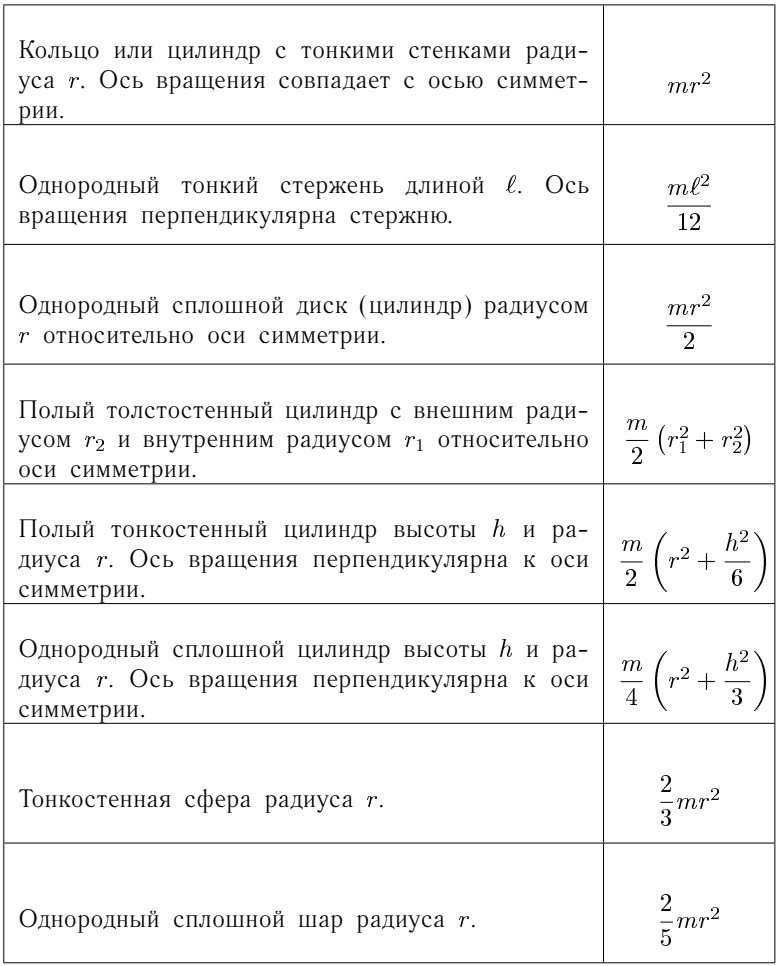
\includegraphics[width=0.9\linewidth]{./formulas}
\end{center}

Занесем результаты в 6 и 7 столбцы таблицы 4.

\section{Расчет погрешностей измерений}

Погрешность рассчитана по методу наименьших квадратов из зависимости $M = -k\cdot \varphi$.

Оценим погрешность момента инерции штанги.
\[\Delta I_{rod} = I_{rod}\sqrt{\left(\frac{\Delta k}{k}\right)^2 + \left(\frac{2\Delta T}{T}\right)^2} = 0,520826 \ \text{г}\cdot\text{м}^2\]
Оценим погрешность периода:
\[\Delta T = \frac{T_{max} - T_{min}}{2} = 0,0217 \ \text{с}\]
Аналогично оценим погрешность косвенного измерения моментов инерции тел из таблицы 4.

\begin{center}
	\begin{tabular}{|l|c|}
		\hline
		\multicolumn{1}{|c|}{Объект } & $\Delta I, \text{г}\cdot\text{м}^2$ \bigstrut\\
		\hline
		Сплошной диск & 0,228 \bigstrut\\
		\hline
		Полый цилиндр & 0,151 \bigstrut\\
		\hline
		Сплошной цилиндр & 0,058 \bigstrut\\
		\hline
		Шар   & 0,197 \bigstrut\\
		\hline
	\end{tabular}%
\end{center}

\section{Графики}

\begin{center}
	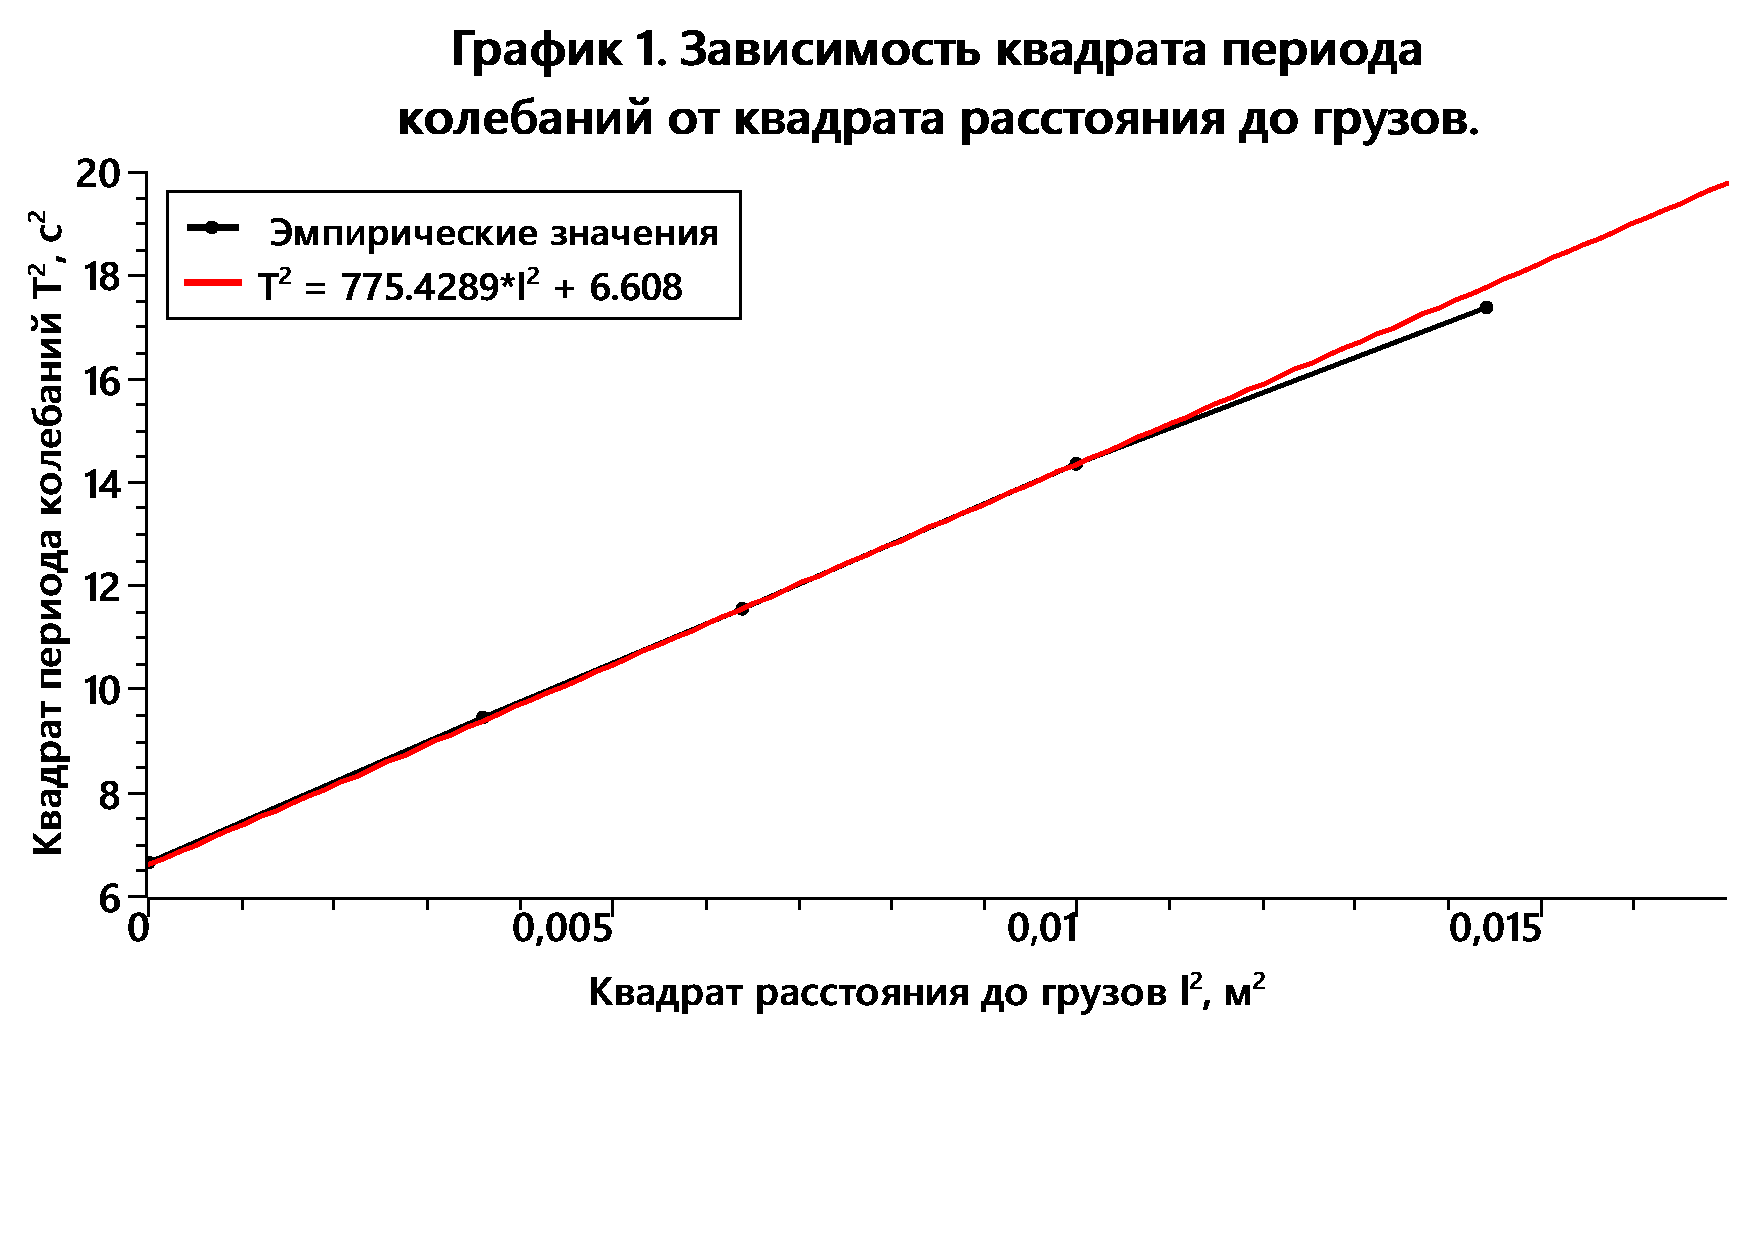
\includegraphics[width=0.8\linewidth]{./picture1}
\end{center}

\begin{center}
	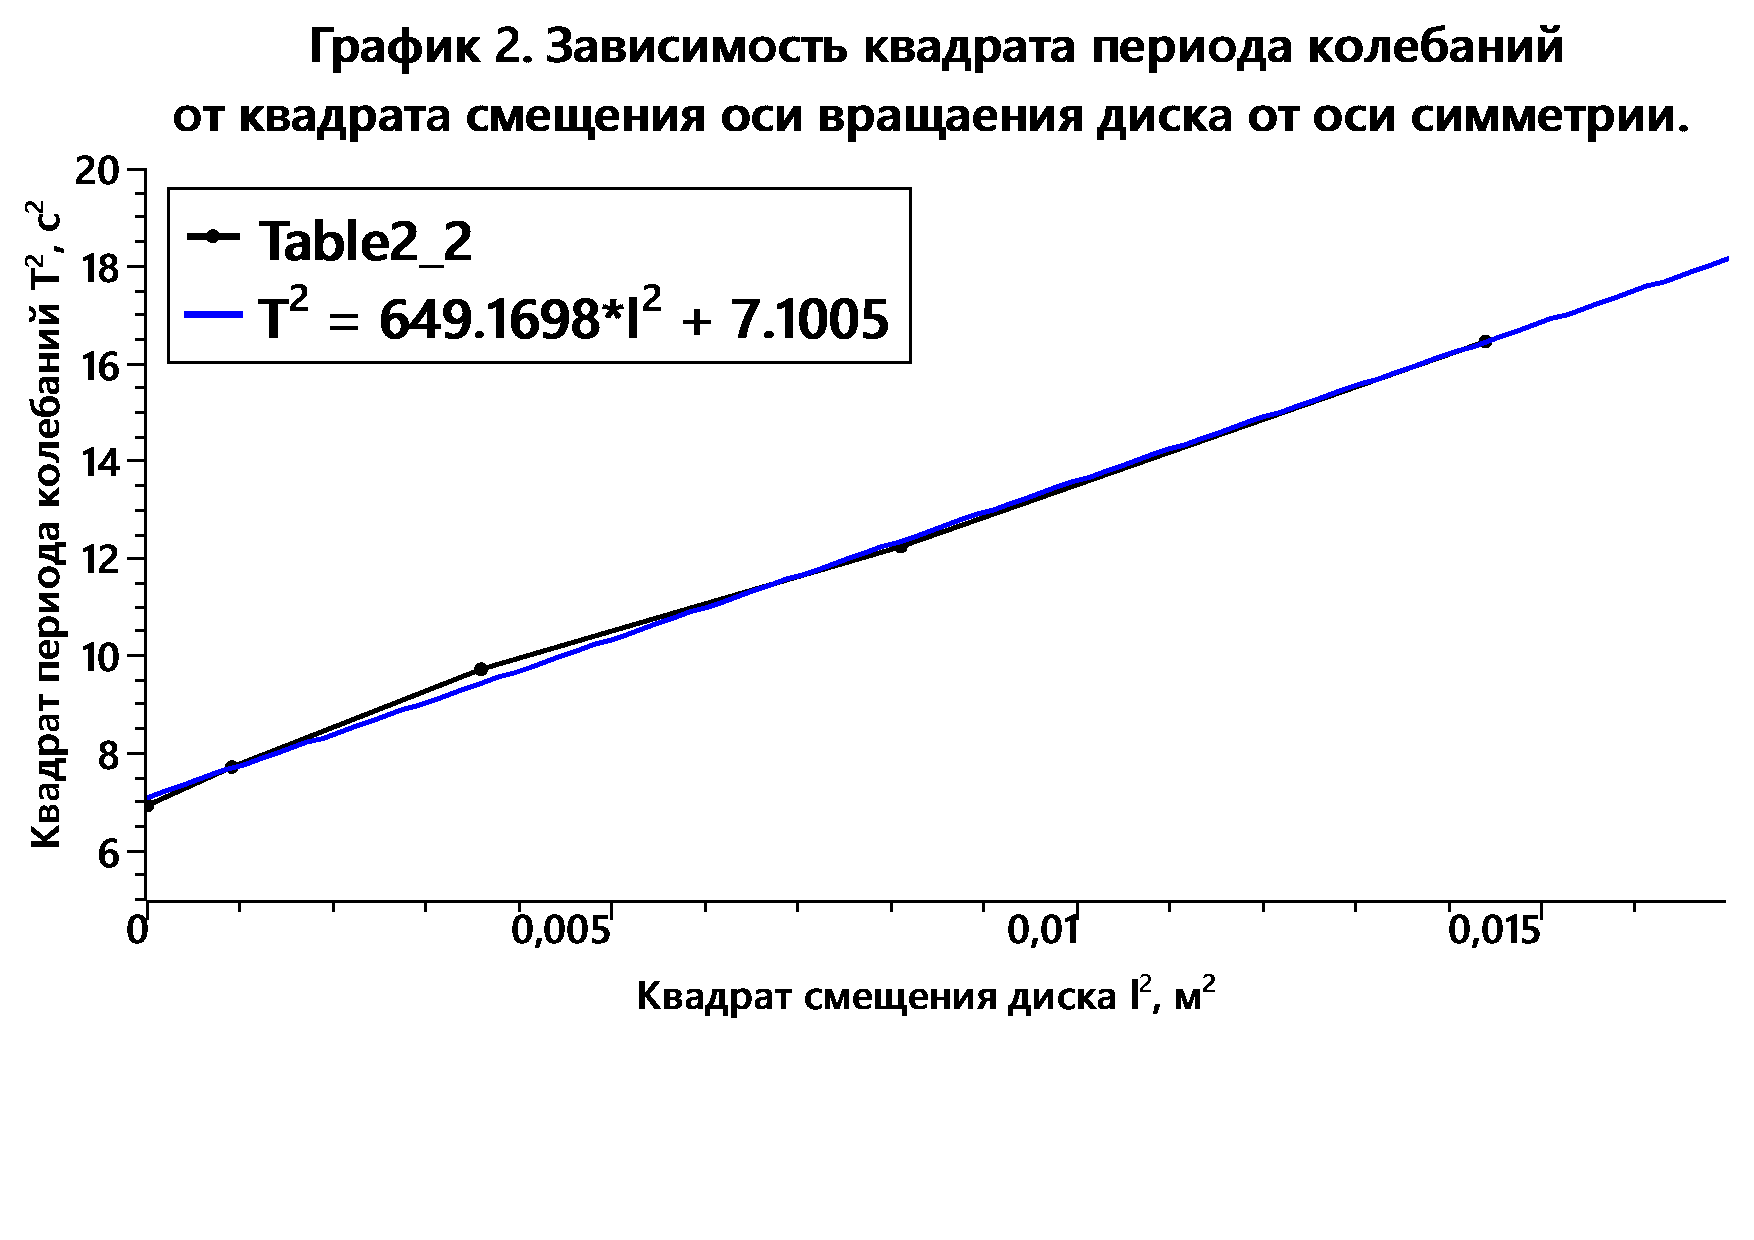
\includegraphics[width=0.8\linewidth]{./picture2}
\end{center}

\section{Окончательные результаты}

\begin{enumerate}
	\item Коэффициент угловой жесткости спиральной пружины.
	\[k = (22,558 \pm 0,972)\cdot 10^{-3} \ \text{Н}\cdot\text{м}\]
	\item Центральный момент инерции штанги.
	\[I_{rod} = 3,816 \pm 0,521 \ \text{г}\cdot\text{м}^2\]
	\[I_{rod, \text{теор}} = 5,250 \ \text{г}\cdot\text{м}^2\]
	\item Масса груза.
	\[m = 221,5 \ \text{г}\]
	\[m_{факт} = 229 \ \text{г}\]
	\item Центральный момент инерции грузов.
	\[I_{c} = 0,115 \ \text{г}\cdot\text{м}^2\]
	\[I_{c, \text{теор}} = 0,134 \ \text{г}\cdot\text{м}^2\]
	\item Центральный момент инерции диска с отверстиями.
	\[I_{c} = 4,057 \ \text{г}\cdot\text{м}^2\]
	\[I_{c, \text{теор}} = 4,939 \ \text{г}\cdot\text{м}^2\]
	\item Центральный момент инерции шара.
	\[I_{c} = 1,347 \pm 0,197 \ \text{г}\cdot\text{м}^2\]
	\[I_{c, \text{теор}} = 1,768 \ \text{г}\cdot\text{м}^2\]
	\item Центральный момент инерции сплошного диска.
	\[I_{c} = 1,372 \pm 0,228 \ \text{г}\cdot\text{м}^2\]
	\[I_{c, \text{теор}} = 1,706 \ \text{г}\cdot\text{м}^2\]
	\item Центральный момент инерции полого цилиндра.
	 \[I_{c} = 0,669 \pm 0,151 \ \text{г}\cdot\text{м}^2\]
	 \[I_{c, \text{теор}} = 0,902 \ \text{г}\cdot\text{м}^2\]
	\item Центральный момент инерции сплошного цилиндра. 
	\[I_{c} = 0,445 \pm 0,058 \ \text{г}\cdot\text{м}^2\]
	\[I_{c, \text{теор}} = 0,581 \ \text{г}\cdot\text{м}^2\]
\end{enumerate}


\section{Выводы и анализ результатов работы}

~

Как видно по графикам зависимости периода колебаний от смещения тел близки к линейным, что говорит о справедливости теоремы Гюйгенса-Штейнера.

Момент инерции большинства исследуемых тел несколько отличается от теоретических значений (примерно на 20\%).
Вероятная причина недостоверности некоторых полученных значений в недостаточно хорошем закреплением оси вращения вместе с телом на установке, из-за люфта смещалось положение равновесия тела относительно пружины.
Результаты оказались занижены, так как из-за плохого закрепления период колебаний уменьшался, и, следовательно, уменьшалось и экспериментальное значение момента инерции тела.

\end{document}
